%%%%%%%%%%%%%%%%%%%%%%%%%%%%%%%%%%%%%%%%%
% Marron Probability Text / Notes
% 
% (from the Science_Textbook_Template)
%%%%%%%%%%%%%%%%%%%%%%%%%%%%%%%%%%%%%%%%%


%----------------------------------------------------------------------------------------
%	PACKAGES AND OTHER DOCUMENT CONFIGURATIONS
%----------------------------------------------------------------------------------------

\documentclass{book}

\usepackage{multicol}
\usepackage{amsmath, amssymb}
\usepackage{tcolorbox}
\usepackage{booktabs}
\usepackage{listings}
\usepackage{courier}   %<== in ./texmf-dist/fonts/type1/adobe/courier

\usepackage[utf8]{inputenc}  
\usepackage{fix-cm}  % this package allows large \fontsize
\usepackage{tikz}    % this is for graphics. e.g. rectangle on title page

% The following dimensions specify 4.75" X 7.5" content on 6 3/8" by 9 1/4"
% paper. The paper width and height can be tweaked as required and the content
% should size to fit within the margins accordingly.
%
% The (inside) bindingoffset should be larger for books with more pages. Some
% standard recommended sizes are .375in minimum up to 1in for 600+ page books.
% Sizes .75in and .875in are also recommended roughly at 150 and 400 pages.
%\usepackage[bindingoffset=0.625in,
%            left=.5in, right=.5in,
%            top=.8125in, bottom=.9375in,
%            paperwidth=6.375in, paperheight=9.25in]{geometry}

% Here is geometry for reading on letter size paper:
\usepackage[margin=.75in, paperwidth=8.5in, paperheight=11in]{geometry}

\renewcommand{\contentsname}{Table of Contents} % default is {Contents}
\usepackage{makeidx}
\makeindex % Initialize an index so we can add entries with \index


\newcommand{\booktitle}{Probability}
\newcommand{\booksubtitle}{A Practical, Systems-Based Approach}
\newcommand{\bookauthor}{Bruce D. Marron}
\newcommand{\authorsubtitle}{UTECA, CDMX}
\newcommand{\booklicense}{Creative Commons Zero 1.0 Universal}


% newcommands embedding other objects (booktitle ==> title, which has actual name of book)
%\makeatletter
%\newcommand{\booktitle}{\@title}
%\newcommand{\bookauthor}{\@author}
%\makeatother
%\title{Probability}
%\author{Bruce D. Marron}


\setlength{\columnsep}{1cm}
\lstset{basicstyle=\footnotesize\ttfamily,breaklines=true}


%----------------------------------------
%	BEGIN DOC
%----------------------------------------
\begin{document}
\frontmatter

% No page numbers on the Frontispiece page
\thispagestyle{empty}


% ---- Title Page ----
% geometry will be restored after title page
\newgeometry{top=1.75in,bottom=.5in}
\begin{titlepage}
\begin{flushleft}

% Title
\textbf{\fontfamily{qcs}\fontsize{48}{54}\selectfont \booktitle}

% Draw a line 4pt high
\par\noindent\rule{\textwidth}{4pt}\\

% Shaded box from left to right with Subtitle
% The text node is midway (centered).

\begin{tikzpicture}
\shade[bottom color=lightgray,top color=white]
    (0,0) rectangle (\textwidth, 1.5)
    node[midway] {\textbf{\large \textit{\booksubtitle}}};
\end{tikzpicture}

% Edition Number
%\begin{flushright}
%\Large 2025
%\end{flushright}

\vspace{\fill}    %fill the extra space

% Author and Title
\textbf{\large \bookauthor}\\[3.5pt]
\textbf{\large \textit{\authorsubtitle}}

\vspace{\fill}

\begin{center}
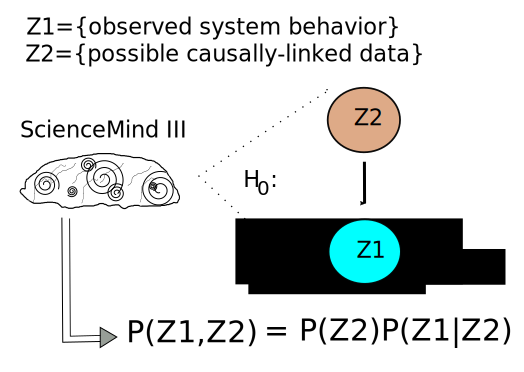
\includegraphics[scale=1.2]{graphics/drawing1b.png}\\[4pt]
%\fontfamily{lmtt}\small{Self Publishers Worldwide\\
%Seattle San Francisco New York\\
%London Paris Rome Beijing Barcelona}
\end{center}

\end{flushleft}
\end{titlepage}
\restoregeometry
% ---- End of Title Page ----



% Do not show page numbers on colophon page
\thispagestyle{empty}

\begin{flushleft}
\vspace*{\fill}   %<== fill to bottom of page then tex

%\vspace{\fill}   <== text then fill to bottom of page
This book was typeset using \LaTeX{} software.\\
Copyright \textcopyright{} \the\year{}  \bookauthor\\
License: \booklicense
\end{flushleft}

% A title page resets the page # to 1, but the second title page
% was actually page 3. So add two to page counter.
\addtocounter{page}{2}

%----- Preface ----------------------------
% The asterisk excludes chapter from the table of contents.
\chapter*{Preface}
This book is dedeicated to hours of NOT understanding probability theory.


% ---------Three-level Table of Contents ----------------
\setcounter{tocdepth}{3}
\tableofcontents

\mainmatter



%--------- Chapter 1 -------------------------
\chapter{Introduction}
Introduction to Probabi;lity Models, 10th edition by Sheldon Ross



\section{Ross Examples}

Suppose that n independent trials, each of which results in any of m possible outcomes with respective probabilities p1 , . . . , pm , $\sum pi = 1$, are continually performed. Let X denote the number of trials needed until each outcome has occurred at least once. Define the equation for X=n and explain the reasoning.\\


Let outcomes be $1,\dots,m$ with probabilities $p_1,\dots,p_m$ (independent across trials). For $n<m$, $\mathbb{P}(X=n)=0$. For $n\ge m$\\

$$
\boxed{\;\mathbb{P}(X=n)=\sum_{\varnothing\neq S\subseteq\{1,\dots,m\}}
(-1)^{|S|+1}\Big(\sum_{j\in S}p_j\Big)\Big(1-\sum_{j\in S}p_j\Big)^{\,n-1}\;}
$$

\textbf{Why this is true (reasoning)}\\

$X=n$ means: after $n-1$ trials at least one outcome is missing, and on trial $n$ the **last** missing type appears for the **first** time. Equivalently, pick any nonempty set $S$ of outcomes and consider the event that **all** outcomes in $S$ have been missing up to time $n-1$ and one of them appears at time $n$. The probability that no outcome from $S$ appears in a given trial is $1-\sum_{j\in S}p_j$. So the chance they are all missing for the first $n-1$ trials and then one of them appears on trial $n$ is

  $$
  \Big(1-\sum_{j\in S}p_j\Big)^{n-1}\Big(\sum_{j\in S}p_j\Big).
  $$
* But these events for different $S$ overlap (inclusion–exclusion fixes the overcount), giving the alternating-sum formula above.


\section*{Coupon Collector Cheat Sheet (General Probabilities)}
\textbf{Problem:} $m$ outcomes with probabilities $p_1,\dots,p_m>0$, $\sum p_i=1$.\\
$X =$ number of trials until \textbf{all outcomes appear at least once}.\\
Define $q_S = \sum_{j\in S} p_j$ for subset $S \subseteq \{1,\dots,m\}$.

\subsection*{Core Formulas}
\begin{tabular}{@{}ll@{}}
\toprule
\textbf{Quantity} & \textbf{Formula} \\
\midrule
PMF ($n\ge m$) & $\displaystyle \mathbb P(X=n)=\sum_{\varnothing\neq S}(-1)^{|S|+1}\,q_S\,(1-q_S)^{n-1}$ \\
CDF & $\displaystyle \mathbb P(X\le n)=\sum_{S}(-1)^{|S|}(1-q_S)^n$ \\
Expectation & $\displaystyle \mathbb E[X]=\sum_{\varnothing\neq S}(-1)^{|S|+1}\frac{1}{q_S}$ \\
Minimum trials & $X_{\min}=m$ \\
Sanity Check & $\mathbb P(X=m)=m!\prod p_i$; $\sum_{n\ge m} \mathbb P(X=n)=1$ \\
\bottomrule
\end{tabular}

\subsection*{Quick Insights}
\begin{itemize}
    \item Tail behavior dominated by largest $1-q_{\{i\}} = 1-\min p_i$; decays geometrically.
    \item Uniform probs: $p_i=1/m \Rightarrow \mathbb E[X]=m H_m \approx m(\ln m+\gamma)$.
    \item Complexity: exact computation $O(2^m)$; feasible for $m\lesssim 20$.
    \item Simulation: use Monte Carlo for large $m$.
    \item First $m$ trials all distinct probability: $m!\prod p_i$.
\end{itemize}

\subsection*{Algorithm (Bitmask / Combinations)}
\begin{enumerate}
    \item Enumerate all non-empty subsets $S$ (bitmask or itertools.combinations).
    \item Compute $q_S = \sum_{j\in S} p_j$.
    \item Plug into PMF or expectation formulas.
    \item Verify probabilities sum to 1 within tolerance.
\end{enumerate}

\subsection*{Python Helper}
\begin{lstlisting}[language=Python]
from itertools import combinations

def coupon_collector_pmf(p, n):
    m = len(p)
    prob = 0.0
    idx = list(range(m))
    for r in range(1, m+1):
        for subset in combinations(idx, r):
            q = sum(p[i] for i in subset)
            prob += ((-1)**(r+1)) * q * (1-q)**(n-1)
    return prob

def coupon_collector_expectation(p):
    m = len(p)
    exp_val = 0.0
    idx = list(range(m))
    for r in range(1, m+1):
        for subset in combinations(idx, r):
            q = sum(p[i] for i in subset)
            exp_val += ((-1)**(r+1)) * (1/q)
    return exp_val

# Example usage:
p = [0.2, 0.3, 0.5]
for n in range(3, 8):
    print(f"P(X={n}) = {coupon_collector_pmf(p, n):.5f}")
print("E[X] =", coupon_collector_expectation(p))
\end{lstlisting}


\subsection{Example 2.5, p. 23}


\subsection{Excessive Elaborations}

\section{Ross Exercises Chapter 1}
\subsection{Examples}
\subsection{Excessive Elaborations}

\section{Third Principles}
\subsection{Examples}
\subsection{Excessive Elaborations}


%------- Chapter 2 ---------------------------------
\chapter{Theory of Numbers}

\section{First Principles}
\subsection{Examples}
\subsection{Excessive Elaborations}

\section{Second Principles}
\subsection{Examples}
\subsection{Excessive Elaborations}

\section{Third Principles}
\subsection{Examples}
\subsection{Excessive Elaborations}


%--------- Chapter 3 ------------------------
\chapter{Irrational and Transcendent Numbers}

\section{First Principles}
\subsection{Examples}
\subsection{Excessive Elaborations}

\section{Second Principles}
\subsection{Examples}
\subsection{Excessive Elaborations}

\section{Third Principles}
\subsection{Examples}
\subsection{Excessive Elaborations}


\foreach \x in {A,B,C,D,E,F,G,H,I,J,K,L,M,N,O,P,Q,R,S,T,U,V,W,X,Y,Z}
    {\index{\x 1}\index{\x 2}}

\backmatter
\addcontentsline{toc}{chapter}{Index}
\printindex
\end{document}
